\documentclass[12pt, xcolor=dvipsnames,svgnames,x11names]{article}
\usepackage{xcolor}
\usepackage{xspace}
\usepackage{url}
\usepackage[colorlinks=true,bookmarks=false,linkcolor=black,urlcolor=blue,citecolor=black]{hyperref}
\usepackage{fancyhdr}
\usepackage[top=1in,bottom=1.2in,left=1in,right=1in]{geometry}
\usepackage{multicol}
\usepackage{pgfplots}
\usepackage{tikz}
\usetikzlibrary{circuits.logic.US, patterns}
\usepackage{mathpazo}
\usepackage{biolinum} 
\usepackage[all]{tcolorbox}
\usepackage{derivative}
\usepackage{../Lectures/rahul_math}
\renewcommand{\familydefault}{\sfdefault}

% --- Custom Color Palette from Image ---
\definecolor{headerRed}{HTML}{A3403D} % Dark red from image top
\definecolor{patternBg}{HTML}{F2D9D7} % Light pinkish bg from image bottom
\definecolor{binaryText}{HTML}{D1A7A4} % Muted color for binary digits

\usepackage{tikz}
\usetikzlibrary{positioning, arrows.meta, shapes.geometric, calc}

% --- Custom Colors ---
\definecolor{lstmBackground}{RGB}{240, 240, 255}
\definecolor{gateGreen}{RGB}{200, 255, 200}
\definecolor{matrixBlue}{RGB}{135, 206, 250}

% --- Background Pattern Setup ---
\usepackage[pages=all]{background}
\backgroundsetup{
scale=1,
color=black,
opacity=1,
angle=0,
contents={%
  \begin{tikzpicture}[remember picture,overlay]
    % Top Header Bar
    \fill[headerRed] (current page.north west) rectangle ([yshift=-1.2cm]current page.north east);
    % Bottom Binary Background
    \fill[patternBg] (current page.south west) rectangle ([yshift=3.5cm]current page.south east);
    % Decorative Line (from image)
    \draw[headerRed, line width=2pt] ([xshift=1in, yshift=-2.5cm]current page.north west) -- ([xshift=8in, yshift=-2.5cm]current page.north west);
    % Binary Text Overlay (Sample)
    \node[anchor=south, binaryText, font=\ttfamily\scriptsize, inner sep=0pt, yshift=1.5cm] at (current page.south) {
        \begin{tabular}{c@{\hspace{0.5em}}c@{\hspace{0.5em}}c@{\hspace{0.5em}}c@{\hspace{0.5em}}c@{\hspace{0.5em}}c@{\hspace{0.5em}}c}
        0 0 0 0 1 1 1 1 0 0 0 0 1 1 0 1 1 1 0 0 0 1 \\
        1 0 0 1 0 1 0 0 0 1 0 0 1 1 0 0 1 0 1 1 \\
        0 0 1 1 0 0 1 0 1 1 1 0 1 1 0 1 0 1 0 0 0 \\
        The University of Alabama in Huntsville
        \end{tabular}
    };
  \end{tikzpicture}
}
}

\newcommand{\hw}{Classwork 09//Markov Decision Process, Remedial for Quiz 3}
\newcommand{\duedate}{April 14, 2026}

\usetikzlibrary{positioning, arrows.meta, shadows}

% --- Header Styling ---
\makeatletter
\renewcommand{\maketitle}{%
    \vspace*{0.2cm}
    \begin{center}
        \begin{tcolorbox}[
            enhanced,
            colback=white,
            colframe=headerRed,
            arc=0mm,
            title={\textcolor{white}{\bfseries \@title}},
            coltitle=white,
            fonttitle=\bfseries\large,
            attach boxed title to top left={xshift=10pt, yshift=-\tcboxedtitleheight/2},
            boxed title style={sharp corners, colback=headerRed, frame hidden}
        ]
        \large
        \vspace{10pt}
\noindent
\begin{tabular}{@{}p{3.5cm}p{6cm}r@{}}
\textbf{Student Name:} & \underline{\hspace{6cm}} & \textbf{Points:} 30 \\
\end{tabular}

\vspace{10pt}

\noindent
\begin{tabular}{@{}p{3.5cm}p{6cm}r@{}}
\textbf{A Number:} & \underline{\hspace{6cm}} & \textbf{Due Date:} \duedate \\
\end{tabular}
        \end{tcolorbox}
    \end{center}
    \vspace{10pt}
}
\makeatother



\pagestyle{fancy}
\fancyhf{}
\lhead{\small CPE 487/587, Spring 2026}
\rhead{\small \textit{\hw}}
\cfoot{\thepage}
\renewcommand{\headrulewidth}{0pt}

\usepackage{booktabs} % For professional lines


% Define a very light gray for the rows
\definecolor{tablegray}{gray}{0.95}

\begin{document}


\title{\hw}
\maketitle



\section{Markov Decision Process (20 Points)}
\label{sec:mdp}

\begin{figure}[htbp]
    \centering
    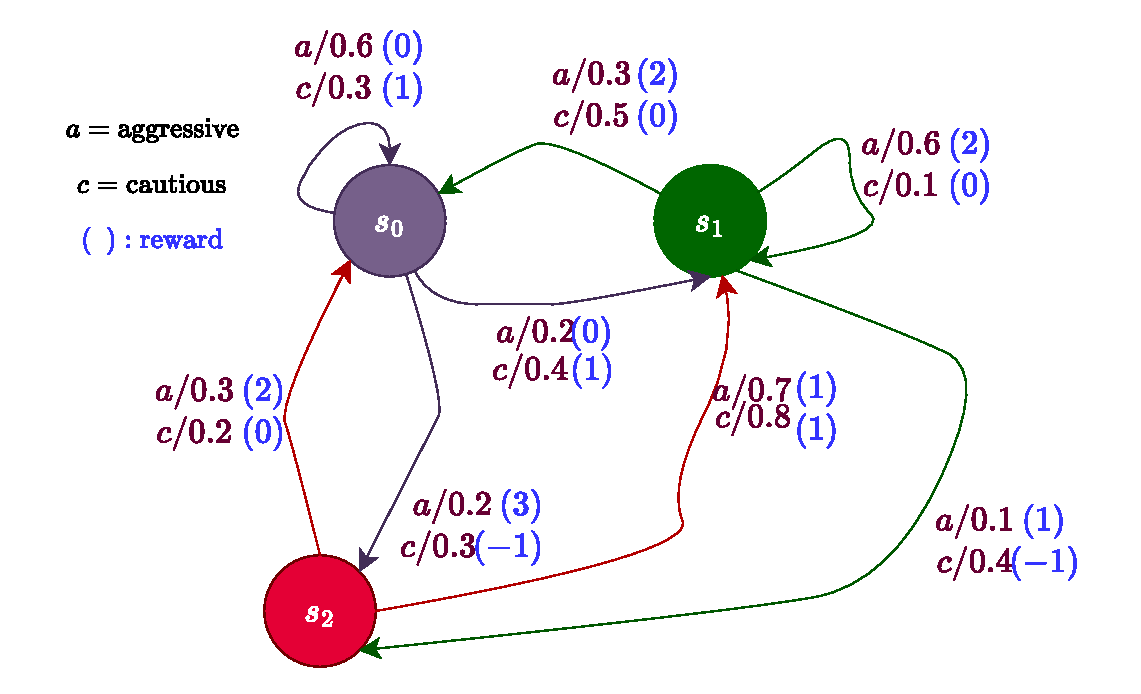
\includegraphics[width=0.90\textwidth]{../Lectures/figures/MarkovChain_WithActionsAndRewardThreeStates.pdf}
    \caption{Q\ref{sec:mdp}}
    \label{fig:mdp}
\end{figure}


\begin{enumerate}

\item Expected immediate reward is given as 

\begin{align*}
\bar{R}(s, a) = \sum_{s'} P(s'|s,a)R(s,a,s')
\end{align*}

Calculate $\bar{R}(s_0, a)$ and $\bar{R}(s_0, c)$. Show your work. \hfill \textbf{(5 Points)}

\item Based solely on expected immediate reward, which action (aggressive or cautious) is preferred in each state? Does the action stay consistent across all three states? \hfill \textbf{(5 Points)}

\item Suppose the agent follows the always aggresive policy $\pi_a$ starting from $s_1$. What is the expected reward after exactly one step? Repeat the same for always-cautious policy $\pi_c$.\hfill \textbf{(5 Points)}

\item Complete the transition table  based on the diagram: \hfill \textbf{(5 Points)}

\begin{table}[htpb]
\centering
\renewcommand{\arraystretch}{1.3}
\begin{tabular}{cccccc}
\hline
\textbf{From} & \textbf{Action} & \textbf{To} & \textbf{Probability} & \textbf{Reward} \\
\hline
$s_0$ & $a$ & $s_0$ & $0.6$ & $0$  \\
$s_0$ & $a$ & $s_1$ & $0.2$ & $0$  \\
$s_0$ & $a$ &  & $0.2$ & $3$  \\
$s_0$ & $c$ & $s_0$ & $0.3$ &   \\
$s_0$ & $c$ &  & $0.4$ & $1$  \\
$s_0$ &  & $s_2$ & $0.3$ & $-1$ \\
\hline
$s_1$ & $a$ & $s_0$ & $0.3$ & $2$  \\
$s_1$ & $a$ &  & $0.6$ & $2$  \\
$s_1$ & $a$ & $s_2$ & $0.1$ & $1$  \\
$s_1$ &  & $s_0$ & $0.5$ & $0$  \\
$s_1$ & $c$ & $s_1$ & $0.1$ & $0$  \\
$s_1$ &  & $s_2$ & $0.4$ & $-1$ \\
\hline
$s_2$ & $a$ & $s_0$ & $0.3$ &    \\
$s_2$ & $a$ &  & $0.7$ & $1$  \\
$s_2$ & $c$ & $s_0$ & $0.2$ & $0$  \\
$s_2$ & $c$ & $s_1$ &  & $1$  \\
\hline
\end{tabular}
\caption{Full transition table. $a = \text{aggressive}$, $c = \text{cautious}$.
         Each row encodes $P(s' \mid s, a)$ and $R(s, a, s')$.}
\label{tab:transitions}
\end{table}




\end{enumerate}


\subsection{Solution}

\begin{enumerate}

\item 


\begin{align*}
\bar{R}(s_0, a) & = \sum_{s'} P(s'|s_0,a)R(s_0,a,s')\\
				& P(s_0|s_0,a)R(s_0,a,s_0) + P(s_1|s_0,a)R(s_0,a,s_1) + P(s_2|s_0,a)R(s_0,a,s_2)\\
				& =  0.6\times 0 + 0.2 \times 0 + 0.2 \times 3 = 0.6
\end{align*}

\begin{align*}
\bar{R}(s_0, c) & = \sum_{s'} P(s'|s_0,c)R(s_0,c,s')\\
				& P(s_0|s_0,c)R(s_0,c,s_0) + P(s_1|s_0,c)R(s_0,c,s_1) + P(s_2|s_0,c)R(s_0,c,s_2)\\
				& =  0.3\times 1 + 0.4 \times 1 + 0.3 \times (-1) = 0.3 + 0.4 - 0.3 = 0.4
\end{align*}


\item 

For state $s_0$, $\bar{R}(s_0, a) > \bar{R}(s_0, c)$, so aggresive action is preferred. 

\begin{align*}
\bar{R}(s_1, c) & = \sum_{s'} P(s'|s_1,c)R(s_1,c,s')\\
				& P(s_0|s_1,c)R(s_1,c,s_0) + P(s_1|s_1,c)R(s_1,c,s_1) + P(s_2|s_1,c)R(s_1,c,s_2)\\
				& =  0.5\times0 + 0.1\times0 + 0.4\times(-1)  = -0.4
\end{align*}

\begin{align*}
\bar{R}(s_1, a) & = \sum_{s'} P(s'|s_1,a)R(s_1,a,s')\\
				& P(s_0|s_1,a)R(s_1,a,s_0) + P(s_1|s_1,a)R(s_1,a,s_1) + P(s_2|s_1,a)R(s_1,a,s_2)\\
				& =   0.3\times 2 + 0.6\times 2 + 0.1\times 1 = 0.6 + 1.2 + 0.1 = 1.9
\end{align*}

For state $s_1$, $\bar{R}(s_1, a) > \bar{R}(s_1, c)$, so aggresive action is preferred. 


%%%%%

\begin{align*}
\bar{R}(s_2, c) & = \sum_{s'} P(s'|s_2,c)R(s_2,c,s')\\
				& P(s_0|s_2,c)R(s_2,c,s_0) + P(s_1|s_2,c)R(s_2,c,s_1) + P(s_2|s_2,c)R(s_2,c,s_2)\\
				& =   0.2\times 0 + 0.8\times 1 = 0.8 
\end{align*}


\begin{align*}
\bar{R}(s_2, a) & = \sum_{s'} P(s'|s_2,a)R(s_2,a,s')\\
				& P(s_0|s_2,a)R(s_2,a,s_0) + P(s_1|s_2,a)R(s_2,a,s_1) + P(s_2|s_2,a)R(s_2,a,s_2)\\
				& =  0.3\times 2 + 0.7\times 1  = 0.6 + 0.7 = 1.3
\end{align*}


For state $s_2$, $\bar{R}(s_2, a) > \bar{R}(s_2, c)$, so aggresive action is preferred. 


\item 


For always aggressive,starting from $s_1$, the one-step expected reward equals $\bar{R}(s_1, a)$  directly:

\begin{align*}
\Ebb[R | s_1, \Pi_a] = 0.6\times 2 + 0.3 \times 2 + 0.1 \times 1 = 1.2 + 0.6 + 0.1 = 1.9
\end{align*}

For always cautious,starting from $s_1$, the one-step expected reward equals $\bar{R}(s_1, c)$  directly:

\begin{align*}
\Ebb[R | s_1, \Pi_c] = 0.1\times 0 + 0.4 \times (-1) + 0.5 \times 0 = -0.4
\end{align*}


\item 


\begin{table}[htpb]
\centering
\renewcommand{\arraystretch}{1.3}
\begin{tabular}{cccccc}
\hline
\textbf{From} & \textbf{Action} & \textbf{To} & \textbf{Probability} & \textbf{Reward} \\
\hline
$s_0$ & $a$ & $s_0$ & $0.6$ & $0$  \\
$s_0$ & $a$ & $s_1$ & $0.2$ & $0$  \\
$s_0$ & $a$ & $\boldsymbol{s_2}$ & $0.2$ & $3$  \\
$s_0$ & $c$ & $s_0$ & $0.3$ & $\boldsymbol{1}$  \\
$s_0$ & $c$ & $\boldsymbol{s_1}$   & $0.4$ & $1$  \\
$s_0$ & $\boldsymbol{c}$   & $s_2$ & $0.3$ & $-1$ \\
\hline
$s_1$ & $a$ & $s_0$ & $0.3$ & $2$  \\
$s_1$ & $a$ & $\boldsymbol{s_1}$   & $0.6$ & $2$  \\
$s_1$ & $a$ & $s_2$ & $0.1$ & $1$  \\
$s_1$ & $\boldsymbol{c}$   & $s_0$ & $0.5$ & $0$  \\
$s_1$ & $c$ & $s_1$ & $0.1$ & $0$  \\
$s_1$ & $\boldsymbol{c}$   & $s_2$ & $0.4$ & $-1$ \\
\hline
$s_2$ & $a$ & $s_0$ & $0.3$ & $\boldsymbol{2}$     \\
$s_2$ & $a$ & $\boldsymbol{s_1}$   & $0.7$ & $1$  \\
$s_2$ & $c$ & $s_0$ & $0.2$ & $0$  \\
$s_2$ & $c$ & $s_1$ & $\boldsymbol{0.8}$   & $1$  \\
\hline
\end{tabular}
\caption{Full transition table. $a = \text{aggressive}$, $c = \text{cautious}$.
         Each row encodes $P(s' \mid s, a)$ and $R(s, a, s')$.}
\label{tab:transitions}
\end{table}

\end{enumerate}




%Write Python Code for the following. Provide your python code hand-written on the paper on an addition sheet.
%
%\begin{enumerate}
%    \item Consider Markov Decision Process given in Figure~\ref{fig:mdp}. Compute the steady-state distribution under action $a$ as well as under action $c$ by solving Eigenvalue problem. (3 Points).
%    \item By randomly transitioning states, simulate the state transition, and compute the simulated  steady-state distribution for each actions. (3 Points).
%    \item Now, consider actions and reward, compute the optimal policy using policy iteration and value iteration. (4 Points).
%\end{enumerate}

\section{Quiz 3 Remedial}

Please go through the solution of Quiz 3 posted on Canvas, and rework on the solution to every problem, and provide justification for the each of the solution. \hfill \textbf{(10 Points)}



\end{document}